%\documentclass{article}
%\usepackage[utf8]{inputenc}
%\usepackage{amsmath}
%\usepackage{natbib}
%\usepackage{graphicx}
%\usepackage{astrojournals} % Necesario para nombres de revistas en luis-ref.bib
%\usepackage[spanish, es-minimal]{babel}
%\usepackage{longtable}
%\usepackage{geometry}
%\usepackage{multirow, array}
%\newlength\figwidth
%\setlength\figwidth{0.48\textwidth}
%\bibliographystyle{apj}


%\title{Catalog of stationary bowshock arcs in the Orion Nebula}

%\author{
  %Alumno: Luis Angel Gutiérrez Soto\\
  %Tutor: Dr. William Henney
%}
%\begin{document}
%\maketitle

%\section{Metodología}
\label{chap:methodology}
Como uno de los objetivos de esta tesis es realizar un catálogo completo de los choques de proa en la Nebulosa de Orión, el primer paso llevado cabo en esta tarea fue la identificación y la busqueda en las imágenes del \textit{HST} descritas en el capítulo anterior, de los arcos de emisión ya conocidos. Entonces un grupo de 6 proplyds llamados; 168-326 (LV1), 167-317 (LV2), 166-316 (LV2b), 163-317 (LV3), 161-324 (LV4) y 158-323 (LV5) detectados y mostrados por  \citet{Laques:1979} fueron buscados e idenficados como parte de este trabajo en las observaciones ya mencionadas, aunque es importante subrayar que Laques \& Vidal no observaron los arcos, estos fueron descubierto hasta la década de los 90. Muchos de estos arcos de emisión fueron reportados en varios artículos de Bally. Algunos aparecen en el artículo de \citet{Bally:2000a} y son los siguientes: w000-400, w005-514, w012-407, w014-414, w030-524, w044-527, w056-519, w069-601, w073-227 y w266-558. Los objetos designados con los nombres desde LL1 a LL7 fueron catálogados por primera vez por \citet{Bally:2001a}. Algunos otros objetos aparecen en una lista presentada por \citet{Bally:2006a}. Estos son los que se llaman LL4, LL5, etc que son los mismos mostrados por Bally \& Reipurth, pero otros objetos también son presentados en este artículo tales como; 4468-605, 116-3101, 203-3039, 261-3018, 305-811, 308-3036 y 344-3020. Dos choques de proa producidos por la interacción de los flujos de dos proplyds son mostrados en \citet{Reipurth:2007}, estos objetos de interacción interproplyd son; 066-652, su choque se genera por la colisión con el viento del proplyd 066-652N y 162-456, el cual interacciona con el proplyd 162-456NE. En un catálogo de \citet{Ricci:2008} muchos proplyds y supuestos proplyds son mostrados. Por mencionar algunos, en esta lista aparecen: 066-3251, 121-434, 124-131 y 178-258. En nuestra busqueda encontramos cerca de 20 objetos nuevos (no reportados antes en la literatura), se podrán ver más adelante donde presentamos el catálogo completo. \\         

Después de haber detectado todos los choques de proa en las ya mencionadas observaciones, se hizo la caracterización de estos objetos es decir, se trazaron la forma de los arcos de los choques de proa estacionarios, usando las herramientas del programa ds9 SAO image,  para medir los radios característicos (\(R_{c}\) y \( R_{0}\)). También se estimaron las distancias (\(D\)) de las fuentes a \thC{}, se determinaron las anchuras (\(h\)) de las cáscaras y se  midieron  los valores de la emisión en las imágenes de las cámaras ACS y WFPC2 y se hicieron la pertinentes calibraciones del flujo.

\section{Formas de los arcos}
\label{sec:arcos}

Como primer paso para caracterizar los arcos de los objetos LL en las afueras de las nebulosa y de los proplyds interiores, se trazaron la forma de los mismos. Para ello establecimos las posiciones donde pensamos que se encuentran los arcos de proa con el proposito de delimitar la cáscara formada por los dos choques (internos y externos) como se puede ver en la figura \ref{fig:arco-LL1}, esto se hizo usando el contraste de brillo entre los choques de proa o las cáscaras y el fondo, debido a que los choques son fuertemente radiativos generando que los arcos sean muy brillantes y esto es lo que vemos en las imágenes, entonces estos argumentos nos dan las pautas para distinguir la emisión en las dos regiones (en la cáscara chocada y en el fondo) y así poder trazar los arcos, este procedimiento es un tanto subjetivo porque es un estimador a simple vista de donde se encuentran los choques. No obstante, para reducir los aspectos subjetivos se implementaron algunas herramientas del ds9 SAO image, para ser más exactos usamos los contornos para trazar los bordes de la cáscara chocada. Además se usaron las imágenes en los diferentes filtros donde se ven mejor los choques para trazar los arcos. Por ejemplo en las regiones internas de la nebulosa se usaron imágenes de \oiii{}~\(\lambda5007\) para trazar algunos arcos debido a la alta ionización del gas en esta zona. Para las regiones externas de la nebulosa donde las líneas de baja ionización de \nii{}~\(\lambda6584\) son importantes se utilizaron imágenes del filtro F658N para trazar la forma de algunos arcos LL. También nos dimos cuenta que algunos arcos se ven muy bien en el continuo así que se usaron imágenes del filtro f647m para este fin, aunque para la mayoría de los casos se usaron las imágenes de \ha{} + \nii{}.\\

Por otro lado, estas estructuras deben cumplir los siguientes criterios para poder ser catálogados como arcos. Primero, en el caso de los proplyds interiores los ejes de los choques deben conicidir con el eje del proplyd y estos deben estar arientados hacia \thC, a excepción de los arcos formados por la interacción de dos proplyds donde se toma como eje de referencia uno de los proplyds y donde el choque está orientado hacia el otro proplyd. Ademas en el caso de los proplyds los arcos tienden a tener formas  semi-circulares entorno a los proplyds. Segundo, en el caso de los objetos LL situados en las regiones mas alejadas de la nebulosa sus arcos tienen forma más hiperbólica y están justo en frente de la estrella presecuencia principal orientados hacia el núcleo de la nebulosa. Ahora, para separar los arcos de los objetos HH se usaron imágenes de diferentes filtros, puesto que como se puede ver en la figura \ref{fig:LL1} del capítulo \ref{chap:introduction} el objeto HH asociado a la estrella T-Tauri de LL1 muestra unos nudos muy brillantes en los diferentes filtros que parecen no seguir la forma del arco de proa. 


\begin{figure}
  \centering
   \includegraphics[width=.6\linewidth]{figuras-tesis/forma-LL1.jpg}
  \caption{Formas de los arcos para LL1. Donde los bordes de los choques están delimitados por los puntos; ``x'', para trazar el borde externo y ``+'', para trazar el borde interno para determinar, la posición de la estrella se usaron pequeños círculos o puntos esto se hizo usando las herramientas del ds9 sao image. Esta imagen es tomada del campo 01 de \citet{Bally:2006a} (ACS-F658N) en el sur-oeste de la Nebulosa de Orión, por tanto es una imagen de \ha{}+\nii{}. }
  \label{fig:arco-LL1}
\end{figure}

\section{Estimación de los parámetros. \(D\), \(R_{0}\) , \(R_{c}\) y \(h_{0}\) }
\label{sec:parametros}

El propósito de trazar los arcos hiperbólicos radica en  que con esta información (coordenadas) fue posible estimar varios parámetros observacionales, que nos permitieran extraer información acerca de los choques. En este orden de ideas, una vez que ya teníamos las posiciones tanto de las componentes de los choques como de la estrella misma se pudo establecer la distancia proyectada \(D\), desde la fuente a \thC{} esta medida nos resultará muy útil como vermos más adelante. De la misma manera se midió \(R_{0}\), este radio lo vamos a definir como la distancia a lo largo del eje de simetría, de la fuente\footnote{La fuente podría ser una estrella T-Taury o un proplyd. Objetos de los cuales se origina el viento interno.} \citep{Robberto:2005}  al borde externo o interno de la cáscara chocada, dependiendo de cual sea el caso. El eje de simetría es la línea proyectada en la dirección en que están orientados los arcos, en la figura \ref{fig:radios} y \ref{fig:anchura} está representada por la línea amarilla. No obstante, hay que aclarar que tenemos dos radios debido a la presencia de un borde externo e interno como ya se ha visto. \\ 

\begin{figure}[htp]
\centering
\begin{tabular}{l l}
(\textit{a}) & (\textit{b})  \\
  \includegraphics[width=0.45\linewidth, trim=40 0.98 40 50, clip]{./figuras-tesis/177-341-Bally-01-images-sin.jpg}&
 \includegraphics[width=0.45\linewidth, trim=40 0.98 40 50, clip]{./figuras-tesis/177-341-Bally-01-images.jpg}\\
\end{tabular}
\caption{(\textit{a}) Proplyd 177-341 ubicado en el sureste de la Nebulosa de Orión. (\textit{b}) Mismo proplyd con una representación de los radios característicos: \(R_{0}(\Out{})\); que es el radio del choque externo, medido a lo largo del eje que va desde el proplyd a \(\theta^1\ \text{Ori}\ \text{C}\), este eje está representado por la línea amarilla. \(R_{c}(\Out{})\) y \(R_{c}(\In{})\); llamados radios de curvaturas, son los radios de los círculos ajustados a partir de los puntos (coordenadas) utilizadas para delimitar los bordes externo e interno de la cáscara chocada. }\label{fig:radios}
\end{figure}

Por otro la lado, se han determinado los radios de curvaturas \(R_{c}\), que en este sentido son los radios de los círculos que se han ajustado, utilizando los puntos con los cuales hemos trazado la forma de los choques (ver figura \ref{fig:radios}), en este sentido se han medido los radios de curvatura para el borde interno y el borde externo de la cáscara chocada y los hemos llamado; \(R_{c}(\Out{})\) y \(R_{c}(\In{})\) respectivamente. Es de notar que la posición de la estrella no corresponde con el centro de los dos círculos que hemos fijado, en otras palabras las posiciones de los centros de los círculos dependen de la forma de los arcos que hemos trazado, es así que estos radios (obtenidos a partir de los cículos ajustados) van a ser un indicador de que tan simétricos son los choques, puesto que como podemos ver en la figura \ref{fig:anchura}, el centro de los círculos no coincide con el eje, entonces estaríamos frente a un caso de un choque que no es rigurosamente simétrico.\\

Siguiendo con la metodología llevada a cabo, otro parámetro que hemos podido estimar ha sido la anchura \(h_{0}\), que como veremos va a ser muy importante para determinar características físicas de los choques. No obstante, \(h_{0}\) la  defineremos como el ancho de la cáscara chocada a lo largo del eje de simetría. Por tanto para determinar éste parámetro hemos hecho lo siguiente: a la distancia que se ha estimado desde el borde externo a la estrella o Proplyd (\(R_{0}(\Out{})\)) le hemos restado el radio del choque interno (\(R_{0}(\In{})\)) (ver figura \ref{fig:anchura}), en esta medida tendremos que la anchura está dada por \(h_{0} = R_{0}(\text{out}) - R_{0}(\text{in})\), que es desde luego también es estimado a lo largo del eje del objeto.

\begin{figure}[htp]
\centering
\begin{tabular}{l l}
(\textit{a}) & (\textit{b})  \\
  \includegraphics[width=0.45\linewidth, trim=40 0.98 30 10, clip]{./figuras-tesis/042-628-Bally_16-images.jpg}&
 \includegraphics[width=0.45\linewidth, trim=40 0.98 30 10, clip]{./figuras-tesis/042-628-Bally_16-images-radii.jpg}\\
\end{tabular}
\caption{(\textit{a}) Proplyd 042-628 y su respectivo choque de proa. (\textit{b}) En esta imagen se puede apreciar el mismo proplyd 042-628  con una representación de la anchura \(h_{0}\) y del radio del choque interno \(R_{0}\) a lo largo del eje proplyd-estrella ionizadora. El eje está representado por la línea amarilla.}\label{fig:anchura}
\end{figure}


\section{Estimación y calibración final del flujo-líneas de emisión en las imágenes del ACS y WFPC2}
\label{sec:clibration-final}

\subsection{Determinación de los valores  de la emisión en las imágenes del ACS y WFPC2 }
\label{sec:brillo-superficial}
Otras de las cosas que hemos realizado con nuestros objetos de estudios, ha  sido determinar el brillo superficial de cada uno de ellos. Una vez que hemos trazado la forma de los arcos hiperbólicos, se han extraído de los campos de Bally (que cubren en su mayoría a la Nebulosa de Orión), pequeñas imágenes FITS que sólo abarcan las regiones donde se encuentran los objetos LL y los proplyds, con el propósito de facilitar las mediciones de los valores de las imágenes. Esto mismo se hizo con los campos de Robberto. Así que usando estás pequeñas imágenes hemos medido los valores de las imágenes\footnote{En el caso de de las campos de Bally los valores de las imágenes tienen unidades de \(\mathrm{electrones~s^{-1}~pixel^{-1}}\) y en caso de las imágenes de Robberto tienen unidades de \(\text{counts}~\text{s}^{-1}~\text{pixel}{-1}\).} en un determinado número de puntos o pixeles a lo largo de diferentes ángulos \(\theta\) en la región chocada y en el fondo, donde se ha supuesto que \(\theta = 0\) corresponde al eje proyectado en el plano del cielo que sigue la dirección en que llegan los fotones ionizantes provenientes de la estrella masiva y todos los demás ángulos \(\theta\) se forman a partir de dicho eje, en sentido contrario a las manecillas del reloj. Para ser más didácticos miremos un caso particular de los resultados de tales mediciones, es así que la figura \ref{fig:brillo-theta} nos muestra los valores en función de \(\theta\) para w005-514, no obstante es de notar que esta gráfica permite ver los valores en el fondo, en la zona chocada y más rigurosamente en el centro de la cáscara. Estas mediciones se hicieron tomando la imágenes de la cámara ACS-F658N y de la misma manera se procedió con las imágenes del WFPC2-F656N \citep{Robberto:2013a}. \\

\begin{figure}[htp]
\centering
\begin{tabular}{l l}
(\textit{a}) & (\textit{b})  \\
  \includegraphics[width=0.5\linewidth, trim=60 10 70 50, clip]{./j8oc01010_wcs/w005-514-Bally_01-arcbright-th.jpg}
& \includegraphics[width=0.5\linewidth, trim=60 10 70 50, clip]{./j8oc01010_wcs/w005-514-Robberto_WFPC2_27_f656n-arcbright-th.jpg}\\
\end{tabular}
\caption{Valores de la emisión o brillo superficial para el proplyd w005-514 en unidades de [\(\text{electrones}~\text{s}^{-1}\)], en función de los ángulos \(\theta\). Los puntos representan los pixeles individuales y los colores representan la distancia con respecto a los arcos (\(z = (R - R_{\text{in}})/(R_{\text{out}} - R_{\text{in}})\)). Las líneas indican las medianas de los valores en el centro de la cáscara y en el fondo y la banda de colores representan el rango entre los cuartiles. Para separar los pixeles de la cáscara del fondo se usaron las coordenada de los bordes internos y externos medidos a partir de la diferencia de contraste en la emisión en las imágenes del \textit{HST}. Ahora con los parámetros circulares; \(\theta\) y radios de los bordes obtenidos de los arcos internos y externos usando dichas coordenadas, se midieron los valores de la emisión para los distintos pixeles en función de tales ángulos. Para (\textit{a}) WCS F658N (\textit{b}) WFPC2 F656N.}\label{fig:brillo-theta}
\end{figure}


Por otro lado también se determinó los valores del brillo superficial en función de la posición con respecto a los arcos, dicha posición se ha escrito de la siguiente forma; \(z = (R - R_{\text{in}})/(R_{\text{out}} - R_{\text{in}})\), que serían los radios relativos a la cáscara, donde \(R\) es la separación radial, \(R_{\text{in}}\) es el radio  desde la estrella al borde externo y \(R_{\text{in}}\) es el radio desde  la estrella al borde interno, es así que la figura \ref{fig:brillo-z} ilustra cuales son los valores para las diferentes radios relativos \(z\). Hay que resaltar que este tipo de gráficas las obtuvimos para cada uno de los choques estacionarios.\\
\begin{figure}[htp]
\centering
\begin{tabular}{l l}
(\textit{a}) & (\textit{b})  \\
  \includegraphics[width=0.5\linewidth, trim=60 10 70 50, clip]{./j8oc01010_wcs/w005-514-Bally_01-arcbright-z.jpg}
& \includegraphics[width=0.5\linewidth, trim=60 10 70 50, clip]{./j8oc01010_wcs/w005-514-Robberto_WFPC2_27_f656n-arcbright-z.jpg}\\
\end{tabular}
\caption{Valores del brillo superficial para el proplyd w005-514 en función de la posición  \(z = (R - R_{\text{in}})/(R_{\text{out}} - R_{\text{in}})\). La líneas indican los valores del brillo para diferentes intervalos de angulos \(\theta\).  Para (\textit{a}) WCS F658N (\textit{b}) WFPC2 F656N.}\label{fig:brillo-z}
\end{figure}

Dado que se tenían los valores de la emisión de los pixeles para las diferentes zonas de los choques hiperbólicos como se mencionó arriba, entonces como siguiente paso se determinaron los valores promedios en la cáscara chocada, en el fondo y en el centro de la cáscara. Para ello se implementaron los conceptos de  estadística robusta, que consistió en determinar el ``trimean'' en las diferentes zonas de nuestros objetos (en la cáscara chocada, en el fondo y en el centro de la cáscara). El trimean es definido como el promedio ponderado de la mediana y los dos cuartiles\footnote{En estadística descriptiva los cuartiles son los tres valores que dividen al conjunto de datos ordenados en cuatro partes porcentuales iguales.}. Entonces de acuerdo a esta definición primero fue necesario encontrar los tres cuartiles de los datos; \(q_{1}\), \(q_{2}\) y \(q_{3}\). Luego con la  ecuación \(\text{TM} = 0.25(q_{1} + 2q_{2} + q_{3})\) se calcularon los trimean o los valores promedios del brillo, para el conjunto de pixeles situados en el intervalo angular \(\theta < 45\) en las regiones ya mencionadas de los objetos LL. Por otro lado se estimó el rango intercuartil el cual es la diferencia entre el tercero y primer cuartil (\(q_{3} - q_{1}\)), con esto obtuvimos una medida de la dispersión de nuestros datos. De la misma manera, es decir usando estadística robusta se determinaron el promedio de los valores del brillo para distintos ángulos \(\theta\) (ver figura~\ref{fig:brillo-theta}) y usando el rango intercuartil estimado para cada ángulo \(\theta\) se determinó la anchura de la distribución, que rescalada nos permitió  estimar la desviación estandar y las incertidumbres para una distribución Gaussiana de nuestro juego de datos. \\
 
Hay que tener en cuenta que los valores determinados para las cáscara incluyen los del fondo, entonces para tener unos valores coherentes del mismo, es decir sólo de la cáscara, le hemos restado los valores del fondo. Es importante mencionar que de la misma manera hemos medido los valores de la emisión de las  imágenes de los viejos  mosaicos de WFPC2, es decir aquellas  observaciones obtenidas con el uso de los filtros F656N (\(\mathrm{\ha~6563~\A{}}\)), F658N (\(\mathrm{\nii~6583~\A{}}\)), f502n (\(\oiii{}~5007~\A{}\)) y del filtro para el continuo f547m.\\

\subsection{Estimación de las constantes de calibración}

\label{sec:const}
En esta parte del trabajo hemos escrito los valores de las emisiones medidos en las observaciones de las respectivas cámaras, en unidades físicas esto es en [\(\mathrm{erg\ s^{-1}\ cm^{-2}\ sr^{-1}}\)]. Como ya se dijo los valores medidos en las imágenes tomadas por la cámara ACS con el fitro F658N tienen unidades de [\(\mathrm{electrones\ s^{-1}}~\text{pixel}^{-1}\)] y las unidades de los valores en las imágenes de WFPC2 con el filtro F656N tienen unidades de [\(\text{counts}\ \text{s}^{-1}~\text{pixel}^{-1}\)], entonces se relizó la respectiva conversión de unidades con el propósito de tener el brillo superficial obtenido a partir de las imágenes de las cámaras ACS y WFPC2 en las mismas unidades físicas.\\

\subsubsection{Estimación de las constantes de calibración de las imágenes de Bally (ACS-F658N) y Robberto (WFPC-F656N)}
\label{sec:acs}

Las estimaciones de las constantes de calibración del flujo en las imágenes del \textit{HST}, se pueden hacer de dos maneras. La primera forma de hacerlo consiste en usar las características de los detectores y los filtros medidos en el laboratorio antes del lanzamiento. Dicho de otra forma, este método se basa en utilizar la información clave que aparecen en los encabezados de las imágenes del \textit{HST}. Esta información es mantenida en los archivos de imágenes después del lanzamiento y puede ser recuperada posteriormente por usuarios externos  a través de un visor de imágenes tal como ds9. La segunda manera de hacerlo consiste en intentar hacer una calibración empírica cuando el instrumento ya está en órbita, mediante la comparación con espectros fotométricos terrestres. El problema de este método es que se requieren demasiados recursos del \textit{HST}, esto quiere decir que toma demasiado tiempo que podrían utilizarse en las observaciones directas. Por otro lado no es muy satisfactorio hacerlo de esta manera debido a las limitaciones de las fuentes de referencia astrónomicas disponibles \citep{McMaster:2008}. Así que en este trabajo se ha inplementado el primer método descrito arriba para hacer las calibraciones de las imágenes de Bally (cámara ACS-F658N) y de Robberto (cámara WFPC2-F656N).\\     

En este orden de ideas, para la estimación de los coeficientes de calibración obtuvimos la información clave para la fotometría, del encabezado de las imágenes FITS a través de ds9. Una de estas informaciones es el PHOTFLAM el cual está definido como la densidad de flujo promedio \(F_{\lambda}\) en unidades de [\(\mathrm{erg~cm^{-2}~\A{}^{-1}~electrones^{-1}}\)] que pruducen 1 cuenta\footnote{Cuentas puede referirse a DN o electrones dependiendo del instrumento.} por segundo en las observaciones del \textit{HST}. Primero determinamos la constante de calibración para las imágenes de la cámara ACS y el filtro F658N. Entonces la metodología empleada sigue el siguiente orden; como se mencionó en la sección~\ref{sec:brillo-superficial} las imágenes están en unidades de [\(\mathrm{electrones~s^{-1}~pixel^{-1}}\)], es así que si se multiplican por el PHOTFLAM (inverse sensitivity), se obtienen unidades de [\(\mathrm{erg\ s^{-1}~cm^{-2}~\A{}^{-1}~pixel^{-1}}\)]. No obstante al multiplicar por la anchura rectangular del filtro nos libramos del término \A{} y al dividir por el área del pixel, información que también se obtuvo del encabezado, vemos que se pueden escribir los valores de las imágenes en unidades de brillo superficial [\(\mathrm{erg~s^{-1}~cm^{-2}~sr^{-1}}\)]. De acuerdo a este análisis se estimó el valor de la constante de calibración del flujo en las unidades adecuadas, que es presentada en la tabla~\ref{tab:table-constans}. Para determinar la anchura del filtro se usó una paquetería de python llamada ``pysynphot'', que al implementarse mostró que la anchura rectangular es 74.9405 \(\text{\AA{}}\), esto se hizo separadamente porque esta información no está incluida en el encabezado de las imágenes FITS.\\

En segundo lugar se determinó el coeficiente de calibración  para las imágenes de \citet{Robberto:2013a} (WFPC2-F656N). Esto se hizo usando el mismo procedimiento descrito arriba (calibración del brillo en las imágenes de Bally), para escribir en unidades de brillo superficial los valores de la emisión \(\ha{}~6563~\A{}\) de estas imágenes. Aunque es de notar que para este caso se obtuvo para la anchura del filtro un valor de 28.34207~\A{}. El coeficiente de calibración resultante se puede ver en la tabla~\ref{tab:table-constans}.\\

\subsubsection{Estimación de las  constantes de calibración de las imágenes de los mosaicos de WFPC2}
\label{sec:wpfc2}
Las imágenes de los viejos mosaicos del WFPC2  obtenidas con el filtro f656n (\(\mathrm{\ha~6563~\AA{}}\)) y el filtro f658n (\(\mathrm{\nii~6583~\AA{}}\)) están unidades de [counts], así que para obtener unidades de brillo superficial, también se estimó el coeficiente de calibración para estas observaciones. Para determinar dichas constantes de calibración se hizo el siguiente análisis; para obtener unidades de [\(\mathrm{count~s^{-1}}\)] hay que  dividir entre el tiempo de exposicón, teniendo en cuenta que las observaciones tomadas con el filtro F656N tiene un tiempo de exposición de 200~s y las del filtro F658N tiene un tiempo de exposición de 500~s. Ahora, si estos valores en unidades de [\(\mathrm{count~s^{-1}}\)], se dividen entre los coeficientes de calibración de \citet{Odell:2009}, los cuales a llamado \(\mathrm{K1_{filter}}\) y respectivamente tienen por valor: \(\mathrm{K1_{F656N} = 1.62}\) y \(\mathrm{K1_{F658N} = 160}\) con unidades de [\(\mathrm{10^{-10}~counts~cm^{2}~sr~phtons^{-1}}\)], se obtienen unidades de [\(\mathrm{photons~s^{-1}~cm^{-2}~sr^{-1}}\)]. Por último, al multiplicar por la energía del fotón (\(\mathrm{E=3.027\times 10^{-12}~erg~para~\ha{}~6563~\AA{}}\) y \(\mathrm{E=3.018 \times10^{-12}~erg}\) para \(\nii{}~6583~\A{}\)) se obtienen cantidades con unidades de [\(\mathrm{erg~s^{-1}}\)  \(\mathrm{cm^{-2}~sr^{-1}}\)] que al final de cuentas es lo que se quiere.  Con este análisis concluimos que al realizar la operación \(\text{E}/(\mathrm{K1_{fiter}}\))  podemos obtener las constantes de calibración deseadas, teniendo en cuenta que hay que dividir previamente los valores de las imágenes entre T (el tiempo de exposición) y donde E es la energía del fotón. En la tabla~\ref{tab:table-constans} se pueden apreciar los valores de los coeficientes para F656N y F658N.


\begin{table}[htp]
\centering
\small\raggedright
\renewcommand{\arraystretch}{1.5}
\caption{Valores de los coeficientes de calibración.}
  \label{tab:table-constans}

\begin{tabular}{ |l| |c| |l| }
\hline
Cámara-filtro&                       Coeficiente de calibración&       Unidades\\ \hline 
ACS-F658N (Imágenes de Bally)&       0.00250 &                          \(\mathrm{erg~electrones^{-1}~cm^{-2}~sr^{-1}}\)\\
WFPC2-F656N (Imágenes de Robberto)&  0.16896 &                          \(\mathrm{erg~counts^{-1}~cm^{-2}~sr^{-1}}\)\\
WFPC2-F656N (Mosaico)&               0.01868 &                          \(\mathrm{erg~counts^{-1}~cm^{-2}~sr^{-1}}\)\\
WFPC2-F658N (Mosaico)&               0.01886 &                          \(\mathrm{erg~counts^{-1}~cm^{-2}~sr^{-1}}\)\\ 
\hline
 \end{tabular} 
 \end{table}
\normalsize

\subsection{Corrección por extinción}
\label{sec:extintion}

Una vez que teníamos los valores fotómetricos y calibrados en flujo, como siguiente paso se realizó la corrección por extinción. Para ello se ha usado un mapa de extinción de \(\text{H}\beta\) junto al siguiente análisis para calcular el flujo correjido por extinción. Entonces para encontrar una expresión del flujo intrísico en términos de la correción \(C_{\text{H}\beta}\) y el flujo observado \(F'\), se ha usado la extinción logarítmica \(C_{\text{H}\beta} = -\log(F'/F) = -\log (\text{exp}(-\tau)) = 0.4343\tau\) (con \(F'/F = \text{exp}(-\tau)\)),  la extinción en magnitud \(A_{\text{H}\beta}=-2.5\log(F'_{\text{H}\beta}/F_{\text{H}\beta})\) para  \(\text{H}\beta\), donde  \(F\) es el flujo intrínsico y \(F'\) es el flujo observado. Y la extinción absoluta  

\begin{equation}
A_{\lambda}=-2.5\log(F'_{\lambda}/F_{\lambda})=2.5C_{\lambda}=1.086\tau
\label{eq:exti}
\end{equation}

Ahora bien, de acuerdo a las anteriores expresiones, la extinción nebular se puede escribir como la extinción logarítmica \(C_{\lambda} = C_{\text{H}\beta}(A_{\lambda}/A_{\text{H}\beta})\), sustituyendo esta última expresión en la Ec. \ref{eq:exti} se obtiene que  \(F_{\lambda} = F'_{\lambda}\times10^{C_{\text{H}\beta}(A_{\lambda}/A_{\text{H}\beta})}\). No obstante si  \(f_{\lambda}= E_{\lambda-\text{H}\beta}/A_{\text{H}\beta}\) como han mencionado \citet{Costero:1970} y dado que \(E_{\lambda-\text{H}\beta}=A_{\lambda}-A_{\text{H}\beta}\), entonces se tendrá que \(f_{\lambda} = (A_{\lambda}/A_{\text{H}\beta})-1\) y esto lleva a concluir que \(C_{\lambda}= C_{\text{H}\beta}(1+f_{\lambda})\). De este modo el flujo corregido por extinción se puede escribe de la siguiente forma

\begin{equation}
  \label{eq:flujo}
  F_{\lambda} = F'_{\lambda}\times10^{C_{\text{H}\beta}(1+f_{\lambda})}
\end{equation}

 Donde se tiene que \(C_{\text{H}\beta}\) es la corrección de enrrojecimiento en \(\mathrm{H\beta}\) y \(f_{\lambda}\) es la función de enrrojecimiento normalizada en \(\mathrm{H\beta}\) con \(f_{\beta}=0.0\) \citep{Peimbert:1977}. Para \(\ha{}~(6563~\A{})\) la función de enrrojecimiento es \(f_{\lambda} = -0.220\) \citep{Blagrave:2007}. Por otro lado \(C_{\text{H}\beta}\) es determinado mediante la comparación del valor teórico esperado para una temperatura y una densidad electrónica con el valor observado de la nebulosa, utilizando el hecho de que el cociente entre dos líneas de recombinación de hidrógeno es casi constante (\citeauthor{Peimbert:1977}). Así que con la Ec. \ref{eq:exti} determinamos el flujo corregido por extinción.

\subsection{Corrección por emisión de \nii{}}
\label{sec:comp}

\begin{figure}[htp]
\centering
\begin{tabular}{l l}
(\textit{a}) & (\textit{b})  \\
  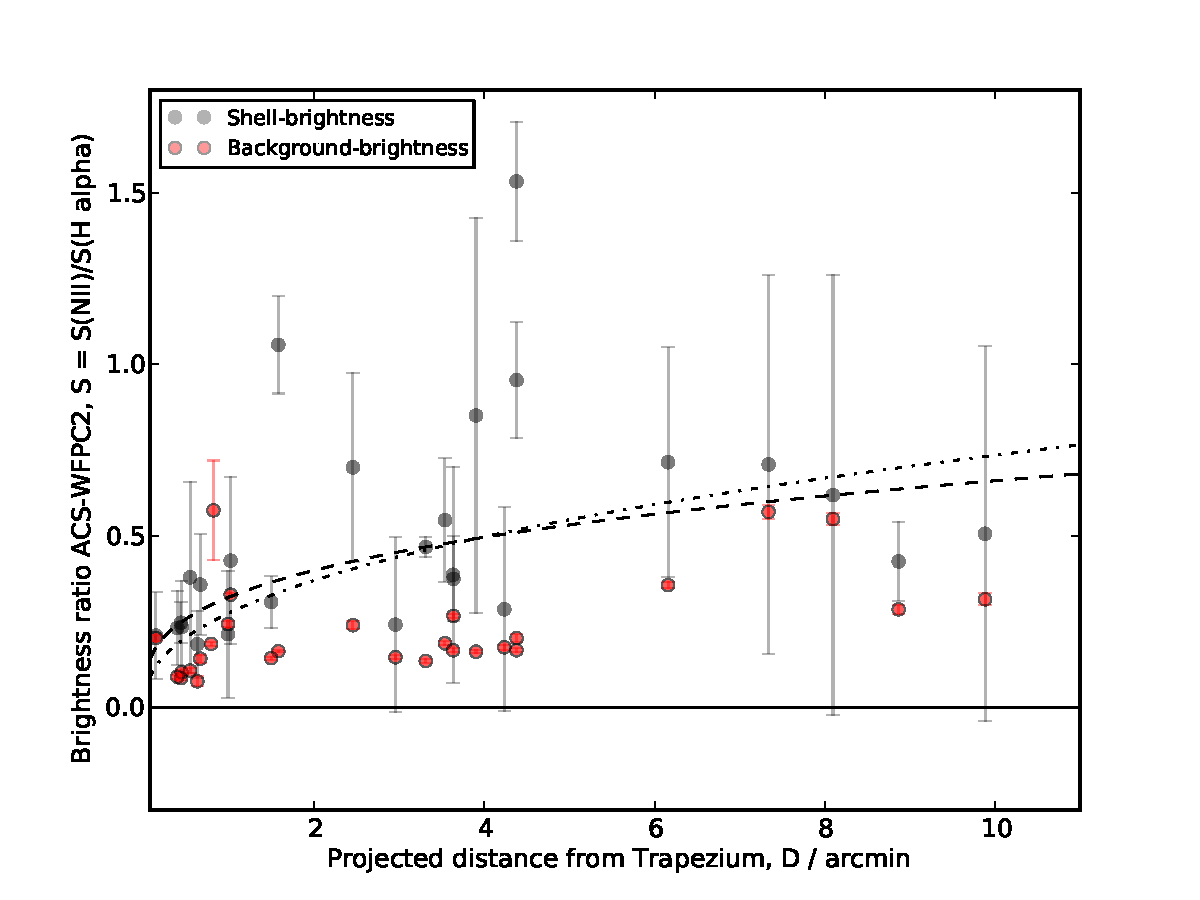
\includegraphics[width=0.48\linewidth, trim=20 9.5 50 20, clip]{./acs_wfpc2-ratio-Nii_ha-vs-D_-mean-error_new}
& 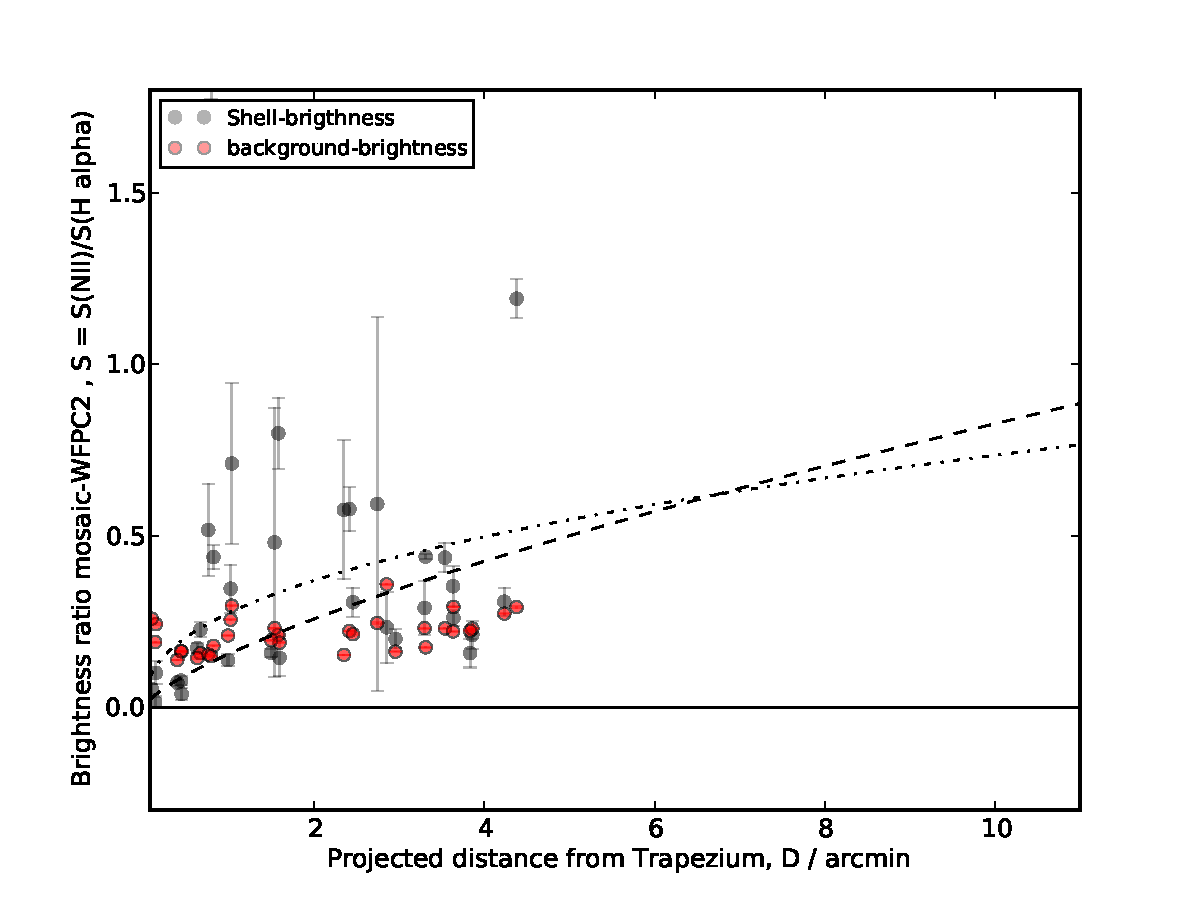
\includegraphics[width=0.48\linewidth, trim=20 9.5 50 20, clip]{./wfpc2-mosaic-ratio-Nii_ha-vs-D_-mean-error_new}\\
\end{tabular}
\caption{Cociente entre el brillo superficial de \nii{} y el brillo superficial de \ha{}, para la cáscara corregida por el fondo (símbolos de color negro) y para el fondo (símbolos de color rojo) en función de la distancia proyectada. (\textit{a}) Usando las observaciones de Robberto, es decir las imágenes de \ha{} de la cámara WFPC2-F656N y las de Bally es decir, las imágenes de \ha{}+\nii{} de la cámara ACS-F658N. La línea discontinua representa un ajuste de un polinomio a los punto graficados la de cáscara chocada cuya relación resultante del ajuste es \(S(\nii{})/S(\ha{})=0.32D^{0.31}\). (\textit{b}) Para el mismo fin se usaron las imágenes de los mosaicos de \ha{} y \nii{} de la cámara WFPC2. La línea discontinua representa lo mismo que en (\textit{a}), pero en este caso son para los datos del mosaico y la relación resultante es \(S(\nii{})/S(\ha{})=0.16D^{0.72}\). La línea de puntos en ambas figuras es un  ajuste  por la combinacion de los dos pares de juegos de datos, esto es, las imágenes de Bally y Robberto con las imágenes de los mosaicos del WFPC2, la relación de este ajuste es \(S(\nii{})/S(\ha{})=0.28D^{0.43}\).}\label{fig:ratio-nii-ha}
\end{figure}

La figura \ref{fig:ratio-nii-ha} nos muestra el cociente de brillo superficial de \nii{} entre el brillo de \ha{} \(S(\nii{})/S(\ha{})\), para la cáscara corregido por el fondo y para el fondo, usando las imágenes de la cámara WFPC2-F656N es decir, el brillo de \ha{} extraido previamente de estas imágenes (observaciones de Robberto) y de la cámara ACS-F658N, es decir imágenes de \ha{}+\nii{} (observaciones de Bally), este cociente se estimó usando la relación \(S(\nii{})/S(\ha{}) = 1 + (S(\ha{}+\nii{}))/S(\ha{})\). Simultaneamente se encontró la fracción \(S(\nii{})/S(\ha{})\) usando las observaciones de dos mosaicos de la cámara WFPC2\footnote{Usando los filtros f656n y f658n.}, puesto que uno de estos mosaicos son imágenes de sólo  \ha{} y el otro son imágenes de sólo \nii{}, esto nos permitió  calcular el cociente de brillo más directamente, debido a que en principio estos datos son más confiables, no obstante el problema de estas observaciones es que sólo incluyen las regiones centrales de la nebulosa. Una vez calculado el cociente de brillo para los dos pares de juegos de datos se compararon los resultados, para poder tener más certeza de nuestras mediciones.\\

En la cáscara corregida por el fondo en las observaciones de los mosaicos, se observa que para los objetos que están más cerca del Trapecio el cociente \(S(\nii{})/S(\ha{})\) es aproximadamente 0.0, indicando que la contribución de \nii{} para la emisión total es del \(0.0\%\), esto es razonable debido a que estos objetos cercanos no emiten en \nii{}, por la alta ionización del material en estas regiones, mientras que los objetos más alejados del Trapecio en las observaciones de Bally y Robberto (las observaciones del mosaico sólo se limitan a las regiones centrales de la nebulosa) nos muestran que este cociente se aproxima a 1.0, indicando por tanto que la contribución de \nii{} al brillo superficial en las regiones más alejadas es decir, de baja ionización es \(\sim 50\%\). En el fondo de la nebulosa, en ambas gráficas de la figura \ref{fig:ratio-nii-ha} se puede ver que en las regiones más cercanas al Trapecio  el cociente \(S(\nii{})/S(\ha{})\) es \(\sim 0.25\), esto se traduce en una contribución del \(20\%\) de la emisión de \nii{} a la emisión total, mientras que los objetos más alejados muestran que este cociente es aproximadamente 0.4, indicando que aproximadamente el 30\(\%\) del brillo  es la contribución de la emisión de \nii{}.     \\

No obstante, en ambas gráficas de la figura también es perceptible un ajuste polinomial del cociente de brillo superficial entre \nii{} y \ha{} en función de la distancia proyectada (línea de discontinua) para los valores de la cáscara chocada, aunque hay una pequeña diferencia entre los ajustes  de los dos pares de juegos de datos, debido a que las obsevaciones de los mosaicos no incluyen los objetos situados en las regiones más alejadas de la nebulosa. Para las observaciones de los mosaicos se realizó una extrapolación del ajuste a esas grandes distancia, aunque esto no brinda mucha confianza si es un indicador de la relación entre el cociente \(S(\nii{})/S(\ha{})\) y la distancia \(D\). Para reducir la discrepancia entre los dos ajuste hicimos un nuevo ajuste pero esta vez combinando los dos pares de juegos de datos (línea de puntos en ambas gráficas), mostrando que este nuevo ajuste presenta la relación \(S(\nii{})/S(\ha{}) \sim D^{0.43}\). Entonces este último ajuste fue el que utilizamos posteriormente para hacer la correción por emisión de \nii{} del brillo superficial de \nii{} + \ha{} en las observaciones de Bally.\\     

%\bibliography{luis-ref}

%\end{document}
